% write document class
\documentclass[12pt]{article}

% write packages
\usepackage{graphicx}
\usepackage{setspace}
\usepackage{booktabs}


% write title, assignment 1, 4 authors and date
\title{\textbf{\Huge CS5600 \\ Assigment 2 } \\ \textbf{Frequent Pattern Mining}}
\author{}
\date{}


\begin{document}
\maketitle

% Group 3
\begin{center}
    \textbf{\Large Group 3} \\
    \textbf{\large Members} \\
\end{center} 

% make name rollnuber table
\begin{center}
\begin{tabular}{ |c|c| }
\hline
\textbf{Name} & \textbf{Roll Number}  \\
\hline
\hline
Kritik Agarwal  & CS23MTECH11009 \\
\hline
Darpan Gaur  & CO21BTECH11004  \\
\hline
Hari Priyanka Allam & CC23M24P100001 \\
\hline
Maloth David  &  	CS21BTECH11035  \\
\hline
\end{tabular}
\end{center}

\newpage

% Exercise 1
\section*{Exercise 1}
Used smpf algorithms Apriori, FPGrowth\_itemsets, and Eclat to compute frequent itemsets for retail1.txt and retail2.txt datasets. \\
\\
Minimum support threshold (0.05\%, 1\%, 2\%, 3\%, 5\%, 7\%). \\

\begin{figure}[h]
    \centering
    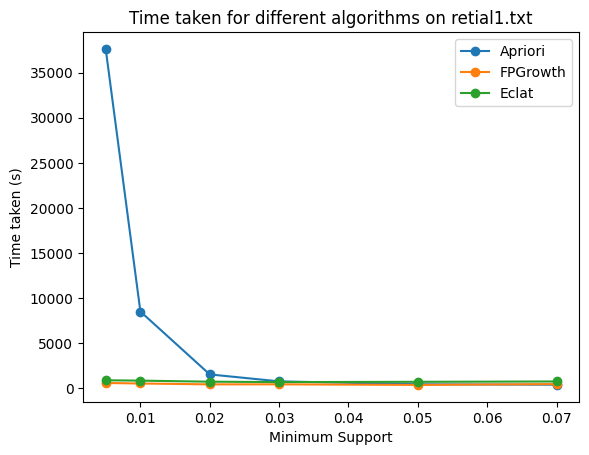
\includegraphics[width=0.8\textwidth]{1a.png}
    \caption{Minimum support vs Computational time for retail1.txt}
\end{figure}

Observations: retail1.txt
\begin{itemize}
    \item For minsup ($<$ 5\%), Apriori performs worst, while FPGrowth\_itemsets performs best, as Apriori use join and prune technique which is computationally expensive.
    \item As minsup increases performance of Apriori improves.
\end{itemize}

\clearpage

% Plot for minimum support vs computational time for retail2.txt.
\begin{figure}[h]
    \centering
    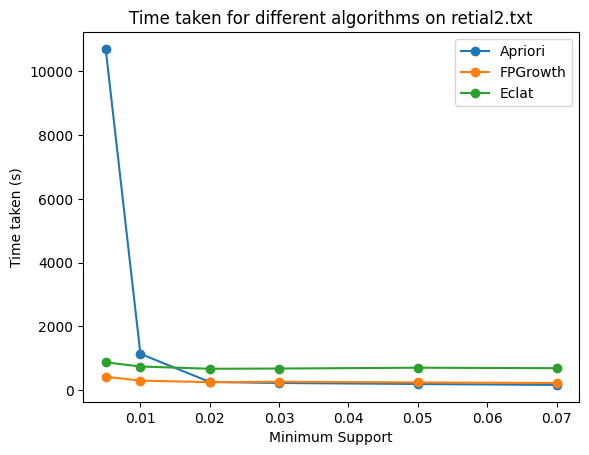
\includegraphics[width=0.8\textwidth]{1b.png}
    \caption{Minimum support vs Computational time for retail2.txt}
\end{figure}
Observations: retail2.txt
\begin{itemize}
    \item Apriori performs worst for minsup (0.05\%, 1\%) and FPGrowth performs best.
    \item Eclat performs worst for minsup ($>$ 2\%), while FPGrowth and Apriori performance are comparable, as with large dataset there is less increament in time with Apriori as compared to Eclat and FPGrowth.
\end{itemize}


% Exercise 2
\section*{Exercise 2}
% make table algorithm vs min-sup
\begin{table}[h]
    \centering
    \begin{tabular}{ |c|c|c|c|c| }
        \hline
        \textbf{Algorithm} & & \textbf{minsup = 0.05\%} & \textbf{minsup = 1\%} & \textbf{minsup = 2\%} \\
        \hline
        \hline
        FPGrowth & Time & 491 & 430 & 419  \\
        % \hline
        & Itemsets & 396 & 140 & 45 \\
        \hline
        FPClose & Time & 491 & 419 & 415 \\
        & Itemsets & 5 & 5 & 5 \\
        \hline
        FPMax & Time & 470 & 451 & 413 \\
        & Itemsets & 5 & 5 & 5 \\
        \hline
        \end{tabular}
    \caption{Time and Itemsets on retail1.txt}
\end{table}

\begin{table}[h]
    \centering
    \begin{tabular}{ |c|c|c|c|c| }
        \hline
        \textbf{Algorithm} & & \textbf{minsup = 0.3\%} & \textbf{minsup = 0.5\%} & \textbf{minsup = 1\%} \\
        \hline
        \hline
        FPGrowth & Time & 393 & 360 & 366  \\
        & Itemsets & 24 & 10 & 5 \\
        \hline
        FPClose & Time & 415 & 379 & 348 \\
        & Itemsets & 5 & 5 & 5 \\
        \hline
        FPMax & Time & 415 & 381 & 338 \\
        & Itemsets & 5 & 5 & 5 \\
        \hline
        \end{tabular}
    \caption{Time and Itemsets on retail1.txt (continued)}
\end{table}

\begin{table}[h]
    \centering
    \begin{tabular}{ |c|c|c|c|c| }
        \hline
        \textbf{Algorithm} & & \textbf{minsup = 0.05\%} & \textbf{minsup = 1\%} & \textbf{minsup = 2\%} \\
        \hline
        \hline
        FPGrowth & Time & 418 & 290 & 246  \\
        % \hline
        & Itemsets & 580 & 159 & 55 \\
        \hline
        FPClose & Time & 443 & 331 & 254 \\
        & Itemsets & 13 & 13 & 13 \\
        \hline
        FPMax & Time & 455 & 325 & 246 \\
        & Itemsets & 13 & 13 & 13 \\
        \hline
        \end{tabular}
    \caption{Time and Itemsets on retail2.txt}
\end{table}

\begin{table}[h]
    \centering
    \begin{tabular}{ |c|c|c|c|c| }
        \hline
        \textbf{Algorithm} & & \textbf{minsup = 0.3\%} & \textbf{minsup = 0.5\%} & \textbf{minsup = 0.7\%} \\
        \hline
        \hline
        FPGrowth & Time & 244 & 220 & 224  \\
        % \hline
        & Itemsets & 32 & 16 & 13 \\
        \hline
        FPClose & Time & 243 & 228 & 229 \\
        & Itemsets & 13 & 13 & 13 \\
        \hline
        FPMax & Time & 233 & 233 & 224 \\
        & Itemsets & 13 & 13 & 13 \\
        \hline
        \end{tabular}
    \caption{Time and Itemsets on retail2.txt (continued)}
\end{table}

\clearpage

% Exercise 3
\section*{Exercise 3}

% Exercise 4
% MSPrior algorithm
\section*{Exercise 4}
\begin{figure}[h] % plot for retail1
    \centering
    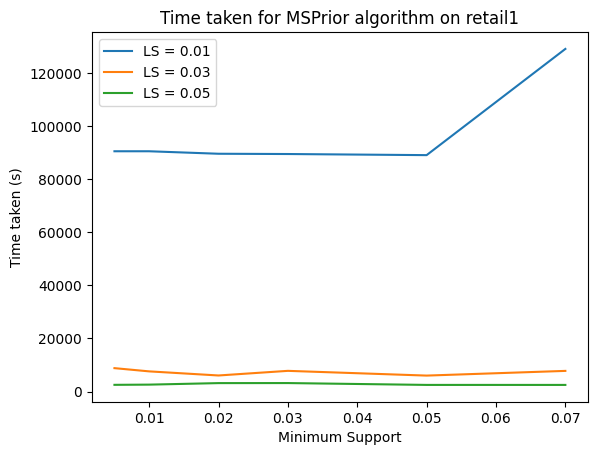
\includegraphics[width=0.8\textwidth]{4a.png}
    \caption{Time taken for MSPrior algorithm on retail1.txt}
\end{figure}

Observations of MSApriori algorithm from SPMF library: retail1.txt

\begin{itemize}
    \item The highest execution times are observed with LS = 0.01 across all minsup values, with times exceeding 89,000 seconds and reaching a peak of 129,007 seconds at minsup = 7\%.
    \item Lower LS values consistently resulted in longer execution times, indicating that a smaller LS results in more granular and intensive processing.
    \item With LS = 0.03 and 0.05, the execution times were significantly lower (e.g., 2,550–8,833 seconds for LS = 0.03 and 2,517–3,199 seconds for LS = 0.05).
\end{itemize}

\begin{table}[h] % time and itemset for retail 1
    \centering
    \begin{tabular}{ |c|c|c|c|c| }
        \hline
        \textbf{LS values} & &  \textbf{minsup = 0\%} & \textbf{minsup = 1\%} & \textbf{minsup = 2\%} \\
        \hline
        \hline
        0.1 & Time(s) & 90481 & 90480 & 89546  \\
        % \hline
        & Itemsets & 140 & 140 & 140 \\
        \hline
        0.03 & Time(s) & 88833 & 7617 & 6072 \\
        & Itemsets & 24 & 24 & 24 \\
        \hline
        0.05 & Time(s) & 2550 & 2628 & 3199 \\
        & Itemsets & 10 & 10 & 10 \\
        \hline
        \end{tabular}
    \caption{Time and Itemsets on retail1.txt}
\end{table}

\begin{table}[h]
    \centering
    \begin{tabular}{ |c|c|c|c|c| }
        \hline
        \textbf{LS values} & & \textbf{minsup = 3\%} & \textbf{minsup = 5\%} & \textbf{minsup = 7\%} \\
        \hline
        \hline
        0.01 & Time(s) & 89441 & 89022 & 129007  \\
        & Itemsets & 140 & 140 & 140 \\
        \hline
        0.03 & Time(s) & 7814 & 379 & 348 \\
        & Itemsets & 24 & 24 & 24 \\
        \hline
        0.05 & Time(s) & 3216 & 2521 & 2517 \\
        & Itemsets & 10 & 10 & 10 \\
        \hline
        \end{tabular}
    \caption{Time and Itemsets on retail1.txt (continued)}
\end{table}

\begin{figure}[h] %plot for retail 2
    \centering
    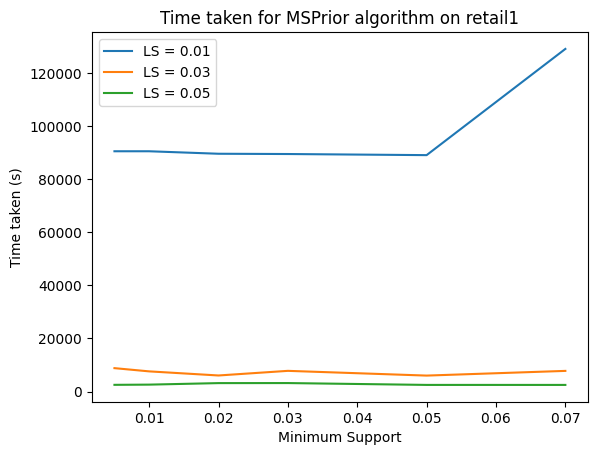
\includegraphics[width=0.8\textwidth]{4a.png}
    \caption{Time taken for MSPrior algorithm on retail2.txt}
\end{figure}

\clearpage

Observations of MSApriori algorithm from SPMF library: retail2.txt[h]
\begin{itemize}
    \item Similar trends were observed, with LS = 0.01 taking the longest time, though the absolute values were lower than retail1.
    \item The execution times for LS = 0.03 and 0.05 were consistently shorter, ranging between 1,141 \em 2,585 seconds for LS = 0.03 and 923 \em 1,165 seconds for LS = 0.05.
\end{itemize}

\begin{table} [h] %time and itemsets for retail2
    \centering
    \begin{tabular}{ |c|c|c|c|c| }
        \hline
        \textbf{LS values} & &  \textbf{minsup = 0\%} & \textbf{minsup = 1\%} & \textbf{minsup = 2\%} \\
        \hline
        \hline
        0.1 & Time(s) & 20400 & 18800 & 16296  \\
        % \hline
        & Itemsets & 159 & 159 & 159 \\
        \hline
        0.03 & Time(s) & 1141 & 1380 & 1231 \\
        & Itemsets & 32 & 32 & 32 \\
        \hline
        0.05 & Time(s) & 1165 & 1088 & 1061 \\
        & Itemsets & 16 & 16 & 16 \\
        \hline
        \end{tabular}
    \caption{Time and Itemsets on retail2.txt}
\end{table}

\begin{table}[h]
    \centering
    \begin{tabular}{ |c|c|c|c|c| }
        \hline
        \textbf{LS values} & & \textbf{minsup = 3\%} & \textbf{minsup = 5\%} & \textbf{minsup = 7\%} \\
        \hline
        \hline
        0.01 & Time(s) & 15609 & 16120 & 14904  \\
        & Itemsets & 159 & 159 & 159 \\
        \hline
        0.03 & Time(s) & 1407 & 1275 & 2585 \\
        & Itemsets & 32 & 32 & 32 \\
        \hline
        0.05 & Time(s) & 1059 & 923 & 1128 \\
        & Itemsets & 16 & 16 & 16 \\
        \hline
        \end{tabular}
    \caption{Time and Itemsets on retail2.txt (continued)}
\end{table}

Number of Itemsets: %comparison[h]
\begin{itemize}
    \item Across both datasets, LS = 0.01 consistently found the most itemsets (140 for retail1 and 159 for retail2), implying more comprehensive mining at a lower threshold.
    \item LS = 0.03 found fewer itemsets (24 for retail1, 32 for retail2), and LS = 0.05 identified the least (10 for retail1, 16 for retail2).
    \item The count of itemsets remained consistent across varying minsup values for each LS, showing stability in the number of frequent itemsets found.
    \item The results indicate that lower LS values lead to longer execution times and more frequent itemsets, reflecting a more thorough analysis of the dataset. However, this comes with a significant computational cost.
    \item Higher LS values (e.g., 0.03 and 0.05) result in shorter execution times and fewer itemsets, suggesting that these configurations may be more suitable for applications requiring faster processing at the cost of finding fewer itemsets.
\end{itemize}

\clearpage
% Exercise 5
\section*{Exercise 5}
\subsection*{Part a}
Cannot-be-together set :- \\ 
\{ \{1543, 1943\} , 
    \{1816, 1834\} , 
    \{225, 1215\} , 
    \{1394, 1989\} , 
    \{1534, 1582\} \}\\
\\
Must-have set :-
\{ \{225\}, 
    \{1394\},
    \{1543\},
    \{1816\},
\}

\subsection*{Part b}

\subsection*{Part c}

\subsection*{Part d}

\end{document}

